\selectlanguage{ngerman}%
\frenchspacing%
\begin{ledgroupsized}[r]{120mm}%
\footnotesize%
\pstart%
\noindent%
\textbf{Überlieferung:}%
\pend%
\end{ledgroupsized}%
\begin{ledgroupsized}[r]{114mm}%
\footnotesize%
\pstart%
\parindent -6mm%
\makebox[6mm][l]{\textit{L}}%
Aufzeichnung:
LH XXXVII\;4 Bl.\;55.
Ein Blatt 4\textsuperscript{o},
Ränder beschnitten;
Papiererhaltungsmaßnahmen.
Drei Viertel Seite auf Bl.\;\href{\Scan{LH_37_04_055r}}{55~r\textsuperscript{o}}.
Bl.\;\href{\Scan{LH_37_04_055v}}{55~v\textsuperscript{o}} überliefert folgenden Entwurf einer Quittung von Leibnizens Hand:
\textit{%
Ich endesbenanter bekenne
daß mir der fürstl. Kämmerer Herr Kuckuck%
\indexN{\textls{Kuckuck} (Guckhguckh), Franz gest. 1702 (?)}
\sout{%
die bereits fallige halbjahrige besoldung dieses iezt lauffenden jahres heut dato baar ausgezahlet,
worüber ihn hiemit zu danck gebührend quittire.
\edlabel{LH_37_04_055_055v_datum-1}%
Hanover den 22 junij Anno Ein tausend Sechshundert Ein und achtzig%
\edlabel{LH_37_04_055_055v_datum-2}%
}
die von Luciae achtzig bis crucis ein und achtzig fallige halbjahrige besoldung mit dreyhundert thalern baar ausgezahlet,
darüber ihn hiemit zu danck gebuhrend quittire.%
} %
Der Rest ist unbeschrieben.%
\pagelabel{LH_37_04_055_uebrlf}
\pend%
\end{ledgroupsized}%
\vspace{5mm}%
\begin{ledgroup}%
\footnotesize%
\pstart%
\noindent%
\textbf{Datierungsgründe:}
Die Datierung der Aufzeichnung N.\;\ref{60234} beruht auf Eigenschaften des Textträgers.
Siehe die ausführliche Begründung auf S.\;\pageref{60234_dat}.%
\pend%
\end{ledgroup}%
\selectlanguage{latin}%
\frenchspacing%
\vspace{8mm}%
\normalsize%
\pstart%
\noindent%
\lbrack%
\href{\Scan{LH_37_04_055r}}%
{55~r\textsuperscript{o}}%
\rbrack%
\hfill%
Pendulae chordae curvitas ex%
\indexS{chorda pendula}%
\indexS{curvitas chordae pendulae}%
\indexS{chorda curva}
\edlabel{LH_37_04_055_055r_ifr-1}%
vibratione%
\indexS{vibratio chordae pendulae}%
\indexS{chorda vibrans}%
\hfill%
\phantom{\lbrack55~r\textsuperscript{o}\rbrack}%
\edtext{}{%
\xxref{LH_37_04_055_055r_ifr-1}{LH_37_04_055_055r_ifr-2}%
\lemma{vibratione}%
\Bfootnote{%
\lbrack/\rbrack\
\textit{(1)}~Die %
\textit{(2)}~Chordam %
\textit{(3)}~Ein strick \textit{ab}%
~\textit{L}%
}}%
\pend%
\vspace{0.5em}%
\pstart%
\noindent%
Ein
\edtext{%
strick \textit{ab}%
\indexS{Strick, schwingend}%
}{%
\lemma{strick \textit{ab}}%
\Cfootnote{%
Vgl.\;das Diagramm \lbrack\textit{Fig.\:1}\rbrack.%
}}%
\edlabel{LH_37_04_055_055r_ifr-2}
welcher an einem orth
\edtext{%
\textit{a}%
}{%
\lemma{\textit{a}}%
\Bfootnote{%
\textit{erg.\;L}%
}}
fest angebunden,
von dannen frey in der lufft%
\indexS{Lufft}
herunter hänget,
und denn
\edtext{%
beweget wird,
daß er%
}{%
\lemma{beweget}%
\Bfootnote{%
\textit{(1)}~werden %
\textit{(2)}~wird, daß %
\textit{(a)}~sie %
\textit{(b)}~er%
~\textit{L}%
}}
hin und hehr
\edtext{%
sich schwinge,%
\indexS{Strick, schwingend}%
}{%
\lemma{sich}%
\Bfootnote{%
\textit{(1)}~schwingen %
\textit{(2)}~schwinge%
~\textit{L}%
}}
bleibet nicht gerade,
sondern machet eine krumme lini,%
\indexS{Linie, krumm}
welche immer krümmer wird,
ie mehr der schwung%
\indexS{Schwung eines hängenden Stricks}
von dem mittel abweichet;
und ob gleich ein gewichte%
\indexS{Gewicht, hängend}
an den strick%
\indexS{Strick, schwingend}
oder faden%
\indexS{Faden, schwingend}
gehänget wird,
so bleibt doch
\edtext{%
diese krümme,%
\indexS{Krümme (Krümmung) eines schwingenden Fadens}
kan also der faden%
\indexS{Faden, schwingend}
eine krümme haben%
\indexS{Krümme (Krümmung) eines schwingenden Fadens}
ob er gleich%
}{%
\lemma{diese krümme,}%
\Bfootnote{%
\textit{(1)}~welche %
\textit{(2)}~ob gleich der faden %
\textit{(3)}~ob er gleich %
\textit{(4)}~kan also %
\lbrack...\rbrack\ er gleich%
~\textit{L}%
}}
frey,
und nicht an herr
\edtext{%
Huygens%
\indexN{\textls{Huygens} (Hugenius, Ugenius, Hugens, Huguens), Christiaan 1629\textendash1695}
Cycloidem%
\indexS{cycloides Hugenii}%
}{%
\lemma{Huygens Cycloidem}%
\Cfootnote{%
Wohl Anspielung auf den geometrischen Nachweis der Tautochronie der Schwingungen eines Zykloidenpendels (bei beliebiger Auslenkung) in
\textsc{C.\;Hyugens},
\textit{Horologium oscillatorium},
pars~II, prop.\;25;
pars~III, prop.\;6
(Paris 1673, S.\;57 u.\;67;\cite{00123}
\textit{HO}\;XVIII, S.\;185 u.\;203).\cite{00113}
}}
oder andere figur%
\indexS{Figur}
anschlägt%
\lbrack;\rbrack\
\edtext{%
stünde demnach zu fragen%
}{%
\lemma{stünde demnach zu fragen}%
\Bfootnote{%
\textit{erg.\;L}%
}}
was dieses für
\edtext{%
eine krumme lini sey,%
\indexS{Linie, krumm}%
}{%
\lemma{eine}%
\Bfootnote{%
\textit{(1)}~figur sey, %
\textit{(2)}~krumme lini sey,%
~\textit{L}%
}}
so der strick macht,%
\indexS{Strick, schwingend}
wenn er gleich durchgehends biegsam;
was auch das ende \textit{b}
im schwingen%
\indexS{Schwingen eines hängenden Stricks}
für eine krumme lini%
\indexS{Linie, krumm}
beschreibe%
\lbrack;\rbrack\
ja wenn der strick%
\indexS{Strick, schwingend}
ungleich biegsam,
\ledpb%
köndte gefragt werden,
mit was graden oder zuwachs
solche biegsamkeit%
\indexS{Biegsamkeit eines schwingenden Stricks}
von einem ende zum andern gehen solte,
damit
sie im schwung%
\indexS{Schwung eines hängenden Stricks}
eine gegebene lini%
\indexS{Linie, krumm}
machen,
oder auch wohl beschreiben könne;
dabey dann auch das gewicht%
\indexS{Gewicht, hängend}
so wohl des stricks selbst,%
\indexS{Strick, schwingend}
als das daran hänget,%
\indexS{Gewicht, hängend}
zu betrachten.
Dieses alles kan ich durch
\edtext{%
meine neue rechnungs%
\indexS{Rechnungs- und Messungsart}
und Meßungs-art,%
}{%
\lemma{meine \lbrack...\rbrack\ Meßungs-art}%
\Cfootnote{Hierbei ist wohl Leibnizens Methode zur Integral- und Differentialrechnung gemeint.}}
ausfinden.
\pend%
\begin{edfigure}[2.50em][0.00em]
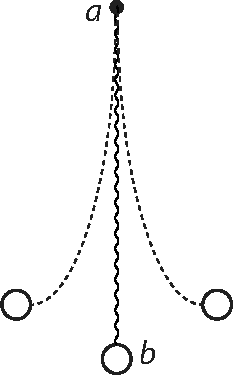
\includegraphics[width=0.18\textwidth]
{gesamttex/edit_VIII-4/images/LH_37_04_055_d_055r.pdf}
\edcaption[0.5em]{\hspace{-1.00mm}\lbrack \textit{Fig.\:1}\rbrack}%
\end{edfigure}%
\vspace{3.0em}%
\pstart%
\noindent%
\centering%
*     *     *
\pend%
\vspace{2.5em}%
\selectlanguage{german}%
\frenchspacing%
\footnotesize%
\pstart%
\noindent%
\textls{Ausführliche Datierungsgründe:}%
\pagelabel{60234_dat}
Der Textträger der undatierten Aufzeichnung N.\;\ref{60234} \textit{Pendulae chordae curvitas ex vibratione} weist kein Wasserzeichen auf, überliefert aber auf der Hinterseite (Bl.\;\href{\Scan{LH_37_04_055v}}{55~v\textsuperscript{o}}) zusätzlich den Entwurf einer Quittung, in der Leibniz bestätigt, vom Hofkammerer Franz Kuckuck\indexN{\textls{Kuckuck} (Guckhguckh), Franz gest. 1702 (?)} für das Halbjahr zwischen Dezember 1680 und Mai 1681 ein Gehalt in Höhe von 300 Reichstaler erhalten zu haben (siehe die Beschreibung der Überlieferung, \pageref{LH_37_04_055_uebrlf}).
Im gestrichenen Textteil des Entwurfs wird die Quittung ausdrücklich auf den 22.\;Juni (2.\;Juli) 1681 datiert; vgl.\;\refpassage{LH_37_04_055_055v_datum-1}{LH_37_04_055_055v_datum-2}.
Die einheitliche Überlieferung rechtfertigt die Annahme, dass auch die Aufzeichnung N.\;\ref{60234} nicht viel früher oder später als den 22.\;Juni (2.\;Juli) 1681 verfasst wurde.
\pend%
\selectlanguage{latin}%
\frenchspacing%
\normalsize%
\newpage%
